\chapter{Fundamentação Teórica}
\label{cap:fundamentacao-teorica}

Este capítulo tem por finalidade apresentar os principais conceitos necessários para o desenvolvimento do presente trabalho. Serão abordados 

\section{Beacons}
\label{sec:beacons}

\cite{Danova} conceitua que beacons são dispositivos de hardware de baixo custo que são pequenos o suficiente para serem fixados em uma parede ou um balcão. Eles utilizam bateria de forma eficiente e conexão bluetooth low energy (de baixo consumo) para enviar mensagens ou notificações para smartphones ou tablets.

\begin{figure}[h!]
	\centering
	\Caption{\label{fig:exemplo-1} Beacons}	
	\UECEfig{}{
		\fbox{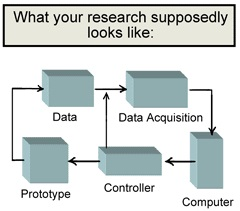
\includegraphics[width=8cm]{figuras/figura-1}}
	}{
	\Fonte{Estimote}			
}	
\end{figure}

\indent Os beacons são considerados dispositivos integrantes da próxima geração da internet, chamada de internet das coisas, onde terão um papel fundamental na forma de comunicação entre as mais variadas instituições como: lojas de varejo, locais de eventos, supermercados, restaurantes e instituições de ensino; e as pessoas. \\
\indent Entre os padrões de beacons existentes atualmente no mercado, dois se destacam por serem desenvolvidos pelas duas empresas -- Apple e Google -- mais importantes e inovadoras da área tecnológica. A seguir, os padrões serão explicados com detalhes. 


\subsection{iBeacon}
\label{sec:ibeacon}

\begin{quote}
O iBeacon é uma nova tecnologia que estende os Serviços de Localização no iOS. Seu dispositivo iOS pode alertar apps quando você se aproxima ou sai de um local com um iBeacon. Além de monitorar um local, o app pode estimar sua proximidade a um iBeacon (por exemplo, uma vitrine ou caixa em uma loja). Em vez de usar latitude e longitude para definir o local, o iBeacon usa um sinal de baixa energia de Bluetooth, detectado pelos dispositivos iOS. \cite{Apple}
\end{quote}

Esta tecnologia foi introduzida pela Apple a partir do seu sistema iOS versão 7, através dela as aplicações podem reagir aos sinal de beacons próximos ao dispositivo do usuário. Para isso o iBeacon envia pequenos pacotes de dados contendo o seu ID e a força de sinal. Como podemos ver abaixo:

\begin{quadro}[h!]	
	\centering
	\Caption{\label{qua:iBeacon-ID} Informações presentes em um pacote de sinal em iBeacons}		
	\UECEqua{}{
		\begin{tabular}{|c|c|l|}
			\hline
			Campo & Tamanho & Descrição \\
			\hline
			UUID & 16 bytes & Número identificador de um conjunto de beacons\\
			\hline
			Major & 2 bytes & Usado para identificar um subconjunto de beacons dentro do conjunto de beacons\\
			\hline
			Minor & 2 bytes & Usado para identificar individualmente um beacon dentro de um subconjunto\\				
			\hline
		\end{tabular}
	}{
	\Fonte{Elaborado pelo autor}
}
\end{quadro}

Os valores contidos no pacote são utilizados de maneira hierárquica pelo sistema iOS para determinar o beacon que o usuário está próximo.

\begin{quadro}[h!]	
	\centering
	\Caption{\label{qua:iBeacon-ID} Hierarquização de informações em iBeacons}		
	\UECEqua{}{
		\begin{tabular}{|c|c|c|c|c|}
			\hline
			\multicolumn{2}{|l|}{Localização} & Manaus & São Paulo & Rio de Janeiro \\
			\hline
			\multicolumn{2}{|l|}{UUID} & \multicolumn{3}{|c|}{AAAAAAAA-BBBB-CCCC-DDDD-EEEEEEEEEEEE}\\
			\hline
			\multicolumn{2}{|l|}{Major} & 1 & 2 & 3\\
			\hline
			\multirow{3}{4em}{Minor} & Bebidas & 10 & 10 & 10\\
			& Higiene & 20 & 20 & 20\\
			& Limpeza & 30 & 30 & 30\\				
			\hline
		\end{tabular}
	}{
	\Fonte{Elaborado pelo autor}
}
\end{quadro}
 
 No quadro acima, está exemplificado o caso envolvendo uma empresa com filiais em três cidades: Manaus, São Paulo e Rio de Janeiro. As três filiais compartilham o mesmo UUID que identifica de forma única a empresa. A identificação de cada filial fica sob responsabilidade do Major; no exemplo 1 para Manaus, 2 para São Paulo e 3 para Rio de Janeiro; E a identificação de cada setor dentro das filiais fica sob responsabilidade do Minor, no exemplo 10 para Bebidas, 20 para Higiene e 30 para Limpeza.
 
 \begin{figure}[h!]
 	\centering
 	\Caption{\label{fig:exemplo-2} Dinâmica do padrão iBeacon}	
 	\UECEfig{}{
 		\fbox{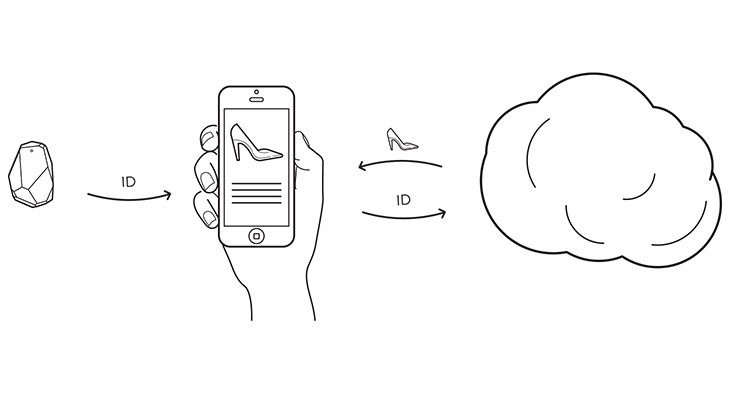
\includegraphics[width=8cm]{figuras/figura-2}}
 	}{
 	\Fonte{Estimote}			
 }	
\end{figure}
 
 \indent Segundo \cite{AppleInsider} iBeacons estão presentes em todas as lojas oficiais da Apple nos Estados Unidos. Através da utilização da aplicação oficial da loja e os iBeacons, os clientes podem ter acesso a uma camada extra de informações e serviços disponíveis nas lojas.
 
 \subsection{Eddystone}
 \label{sec:eddystone}
 
 Eddystone é um formato de beacon aberto do Google e que funciona com os sistemas Android e iOS. Eddystone inclui três tipos de estrutura para transmissão de dados, adequados para diferentes cenários. \cite{Google} \\
 \indent O padrão Eddystone é uma parte integrante da plataforma de beacons da Google. Com sua utilização é possível:
 
 \begin{itemize}
 	\item Permitir que as aplicações reajam ao contexto do usuário através de anexos (attachments) beacons;
 	\item Monitorar o status de uma frota de beacons a estrutura de telemetria do padrão Eddystone;
 	\item Transmitir dados para utilização da Web Física.
 \end{itemize}
 
 \begin{figure}[h!]
 	\centering
 	\Caption{\label{fig:exemplo-3} Dinâmica do padrão Eddystone}	
 	\UECEfig{}{
 		\fbox{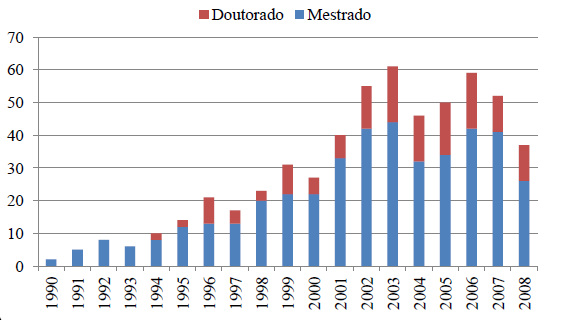
\includegraphics[width=8cm]{figuras/figura-3}}
 	}{
 	\Fonte{Google Developers}			
 }	
\end{figure}

A plataforma de beacons do Google é composta pelos próprios beacons, pelo padrão Eddystone e pela API de proximidade de beacons. \\
\indent Os beacons que suportam as especificações do padrão Eddystone podem transmitir dados de um único tipo de estrutura ou intercalar entre uma estrutura e outra. Por exemplo, transmitir repetidamente 50 estruturas do tipo Eddystone-UID seguidas de uma estrutura Eddystone-TLM. \\
\indent O padrão Eddystone especifica atualmente três tipos de estruturas: Eddystone-UID, Eddystone-URL e Eddystone-TLM.

\subsubsection{Eddystone-UID}
\label{sec:eddystone-uid}

Eddystone-UID contém o número identificador do beacon, que pode ser utilizado por um aplicação para disparar uma ação para o usuário. No Eddystone-UID, assim como ocorre no iBeacon, também é enviado um pequeno pacote de dados contendo um namespace e instance, detalhes no quadro abaixo:

\begin{quadro}[h!]	
	\centering
	\Caption{\label{qua:eddystone-UID} Informações presentes em um pacote de sinal em Eddystone}		
	\UECEqua{}{
		\begin{tabular}{|c|c|l|}
			\hline
			Campo & Tamanho & Descrição \\
			\hline
			Namespace & 10 bytes & Identificador de um conjunto de beacons\\
			\hline
			Instance & 6 bytes & Usado para identificar individualmente um beacon\\
			\hline
		\end{tabular}
	}{
	\Fonte{Elaborado pelo autor}
}
\end{quadro}

Para gerar um namespace a especificação do padrão Eddystone recomenda utilizar os dez primeiros bytes do hash SHA-1 gerado a partir de um nome de domínio. Exemplo de namespace gerado a partir do domínio ``fucapi.br'' utilizando a linguagem python:

\begin{figure}[h!]
	\centering
	\Caption{\label{fig:codigo-3} Código de exemplo para geração de namespace em python}	
	\UECEfig{}{
		\fbox{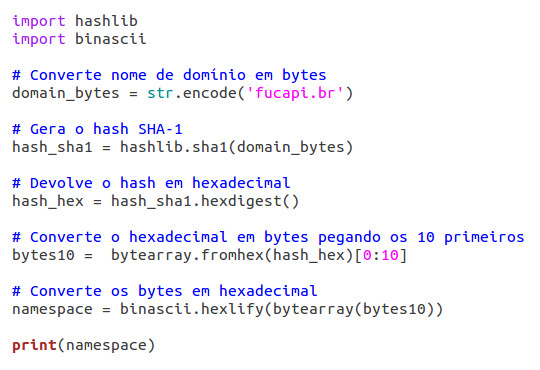
\includegraphics[width=8cm]{figuras/namespace_python}}
	}{
	\Fonte{Elaborado pelo autor}			
}	
\end{figure}

Ao executar o código a saída é:\\
\indent 1755ba6780003245d85c

\subsubsection{Eddystone-URL}
\label{sec:eddystone-url}

Eddystone-URL é a base para um novo conceito criado pela Google, chamado de Web Física, onde o usuário não precisará de um aplicativo dedicado para interpretar e executar as ações ao utilizar beacons fixados em objetos do mundo real. O conteúdo transmitido pelos beacons segue o mesmo padrão das URLs interpretadas pelos navegadores web, assim o usuário poderá acessar o conteúdo -- em forma de webapp ou website -- sem precisar baixar e instalar um aplicativo dedicado.

\subsubsection{Eddystone-TLM}
\label{sec:eddystone-tlm}

Eddystone-TLM especifica uma estrutura apropriada para transmissão de dados sobre os próprios beacons, permitindo que os mesmos possam ser gerenciados. Essa estrutura pode ser enviada juntamente com Eddystone-UID ou Eddystone-URL. A aplicação utilizada pelo usuário deve ser preparada para retransmitir os dados enviados pelo Eddystone-TLM para um serviço externo responsável por prover dados de gerenciamento. \\
\indent A estrutura pode conter os seguintes dados sobre os beacons:      

\begin{itemize}
	\item Tensão da bateria, que pode ser usado para estimar o nível de bateria restante em um beacon;
	\item Temperatura do beacon;
	\item Número de pacotes enviados desde a última vez que o beacon foi ligado ou reiniciado;
	\item Tempo de atividade desde a última vez que o beacon foi ligado ou reiniciado.
\end{itemize}

\section{Raspberry Pi}
\label{sec:raspberrypi}

De acordo com a \cite{RPiFoundation} Raspberry Pi é um microcomputador de dimensões mínimas, semelhante ao tamanho de um cartão de crédito, que pode ser conectado a um monitor e usa teclado e mouse padrão. \\

\begin{figure}[h!]
	\centering
	\Caption{\label{fig:raspberrypi} Raspberry Pi}	
	\UECEfig{}{
		\fbox{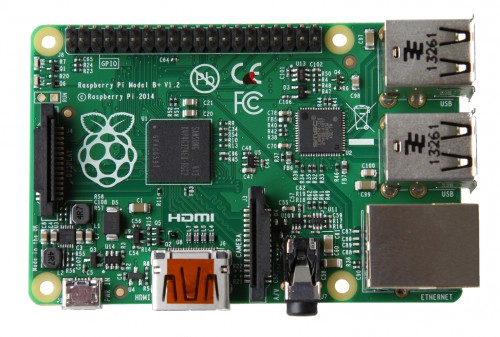
\includegraphics[width=8cm]{figuras/raspberrypi}}
	}{
	\Fonte{Raspberry Pi Foundation}			
}	
\end{figure}

Apesar de ser um microcomputador, é possível realizar a maioria das atividades da mesma forma que são realizadas em um computador pessoal convencional. Como navegar na internet, ouvir arquivos de audio e visualizar videos, criar documentos de textos, planilhas e apresentações. Raspberry Pi é desenvolvido pela Raspberry Pi Foundation, instituição que tem como principal objetivo, promover o estudo da ciência da computação e assuntos relacionados. \\
\indent Atualmente, em sua mais nova versão -- Raspberry Pi 2, é possível utilizar tanto sistema Linux, quanto Windows. Oficialmente é fornecida uma distribuição baseada no linux Debian chamada Raspbian, no caso do Windows a própria Microsoft disponibiliza uma versão adaptada do Windows 10, chamada Windows 10 IoT (Internet of Things). \\
\indent Além das dimensões mínimas, suas principais características estão relacionadas ao processador, armazenamento e porta GPIO (General Purpose Input/Output). O processador é baseado na arquitetura ARM, a mesma presente nos processadores de smartphones e tablets, o que proporciona baixo consumo de energia e também baixo aquecimento ao ponto de não necessitar de um dissipador de calor. O armazenamento de dados, inclusive do sistema operacional, é feito através do uso de um cartão SD, essa forma é muito vantajosa para realização de backup do sistema e também trocar ou alternar rapidamente o sistema utilizado no microcomputador. A porta GPIO é composta por um conjunto de pinos programáveis que são responsáveis pela comunicação de entrada e saída de sinais digitais, através dela é possível fazer comunicação com equipamentos externos ou periféricos. Como por exemplo LEDs, motores, sensores, entre outros.